\begin{minipage}{0.55\textwidth}
    \begin{figure}[h]
    \centering
    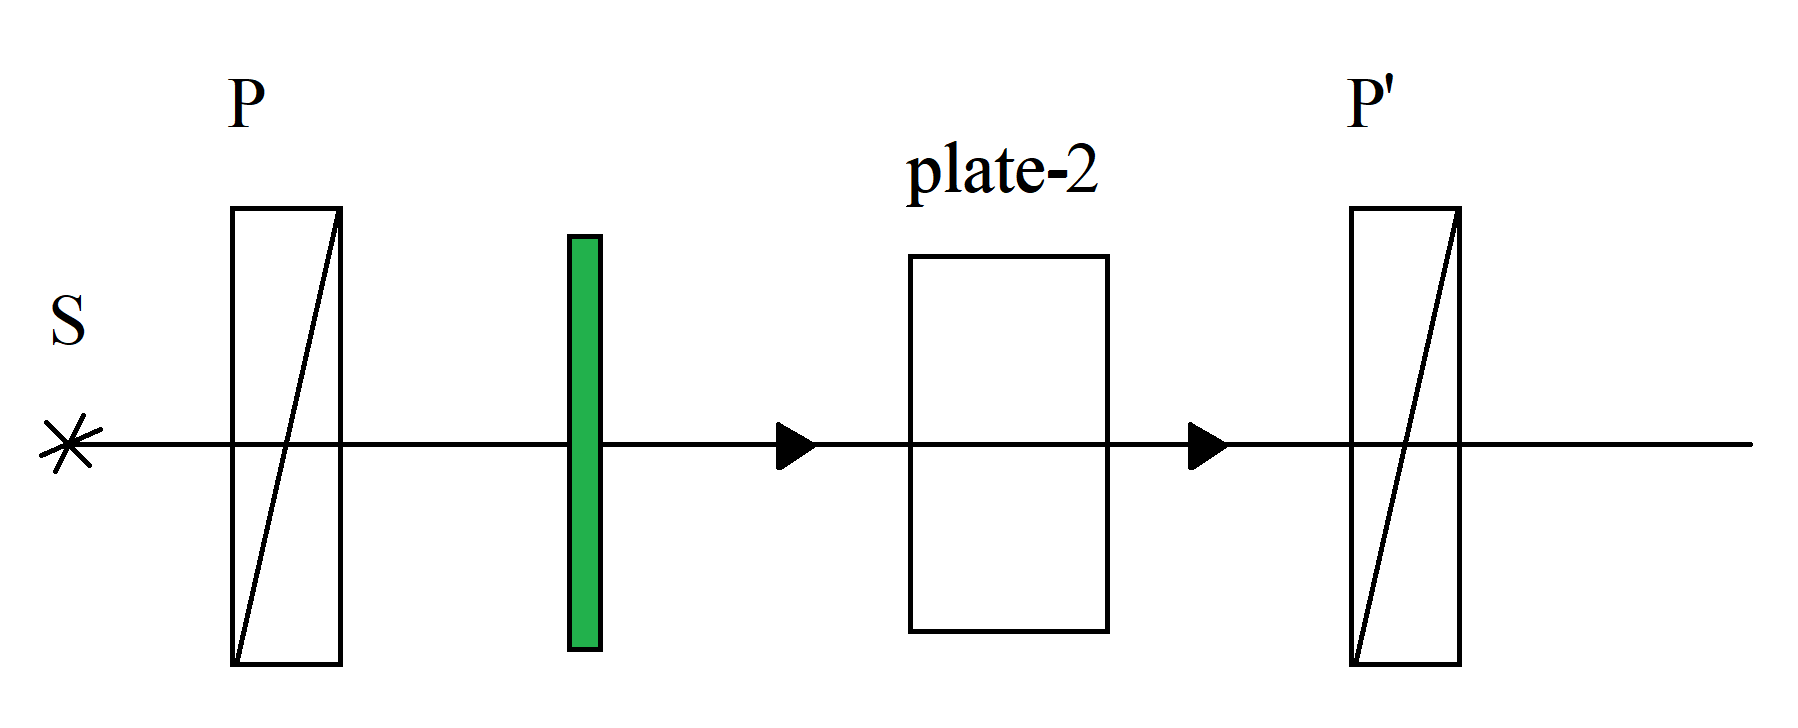
\includegraphics[width=1\textwidth]{images/greeeeeen2.png}
    \caption{To the previous setup we add a green light-filter. And rotate the first polaraid so it is horizontal and the plate is  angled as $45^\circ$.}
    %\label{fig:}
\end{figure}
\end{minipage}
\hfill
\begin{minipage}{0.35\textwidth}
    By rotating the polaroid we obtain that plate-2 is $\lambda/2$, due to observing just fluctuating of its intensity. So no color changing here, no magical video then.
\end{minipage}